\documentclass{beamer}
\usepackage{pgfpages}
\usepackage{xcolor}
\usepackage{graphicx}
\usepackage{caption}

% TikZ
\usepackage{physics}
\usepackage{amsmath}
\usepackage{tikz}
\usepackage{mathdots}
\usepackage{yhmath}
\usepackage{cancel}
\usepackage{color}
\usepackage{siunitx}
\usepackage{array}
\usepackage{multirow}
\usepackage{amssymb}
\usepackage{gensymb}
\usepackage{tabularx}
\usepackage{booktabs}
\usetikzlibrary{fadings}
\usetikzlibrary{patterns}
\usetikzlibrary{shadows.blur}
\usetikzlibrary{shapes}

\usetheme[sectionpage=simple,block=fill]{metropolis}
% \setbeameroption{show notes on second screen}

\definecolor{ured}{HTML}{CC0000}
\definecolor{ugray}{HTML}{808080}
\setbeamercolor{title separator}{fg=ured}
\setbeamercolor{frametitle}{bg=ured}

\title{Introduction to Automating System Builds, Workflows, and Configuration Management with GitHub Actions}
\date{June 29, 2021}
\author{Emerson Ford}
\institute{University of Utah --- ITX Meeting}

\begin{document}
\maketitle

\begin{frame}{Overview}
    \begin{itemize}
        \item Understanding automation
        \item How to automate with Github Actions
        \item Best practices of automation
        \item Q\&A and related topics
    \end{itemize}
\end{frame}

\begin{frame}{What is automation?}
    Getting computers do things for you automatically
    \begin{itemize}
        \item building, testing, and publishing artifacts
        \item linting and auto formatting code
        \item deploying configurations
        \item welcome new contributors to your repo \begin{minipage}{\linewidth}\vspace{2pt}
\includegraphics[width=0.8\linewidth]{welcome.png}\end{minipage}
    \end{itemize}
\end{frame}

\begin{frame}{Why automate?}
    \begin{itemize}
        \item saves you time and headaches
        \item ensure consistent workflow runs
        \item improve visiblity, handoff, and usability
        \item it scales
    \end{itemize}
\end{frame}

\begin{frame}[plain]
    \begin{minipage}{\textwidth}
        \centering
        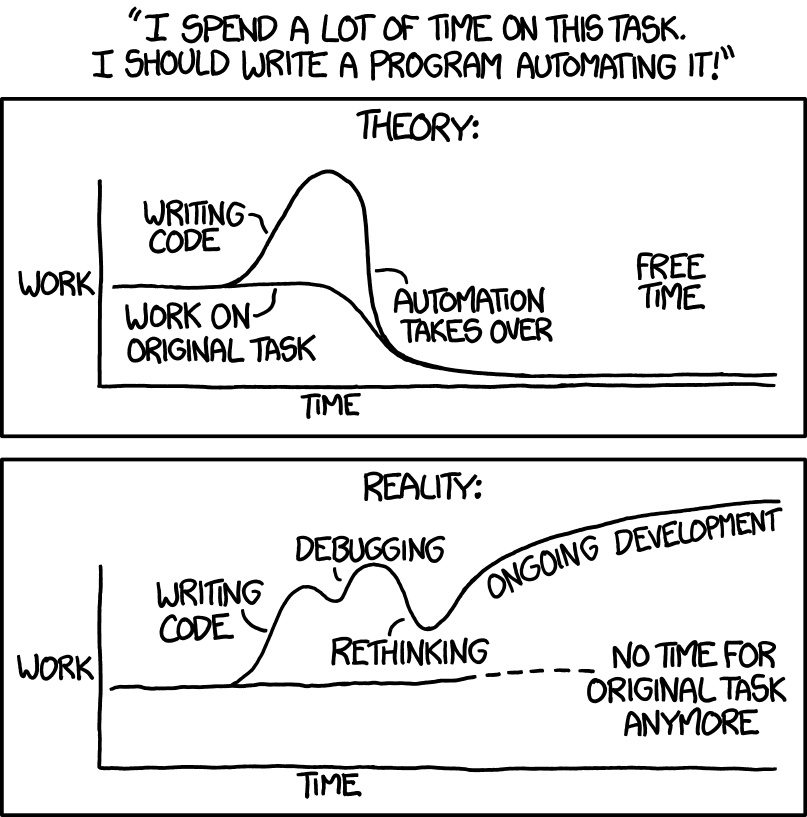
\includegraphics[width=0.7\linewidth]{automation_2x.png}
    \end{minipage}
\end{frame}

\begin{frame}[plain]
    \begin{minipage}{\textwidth}
        \centering
        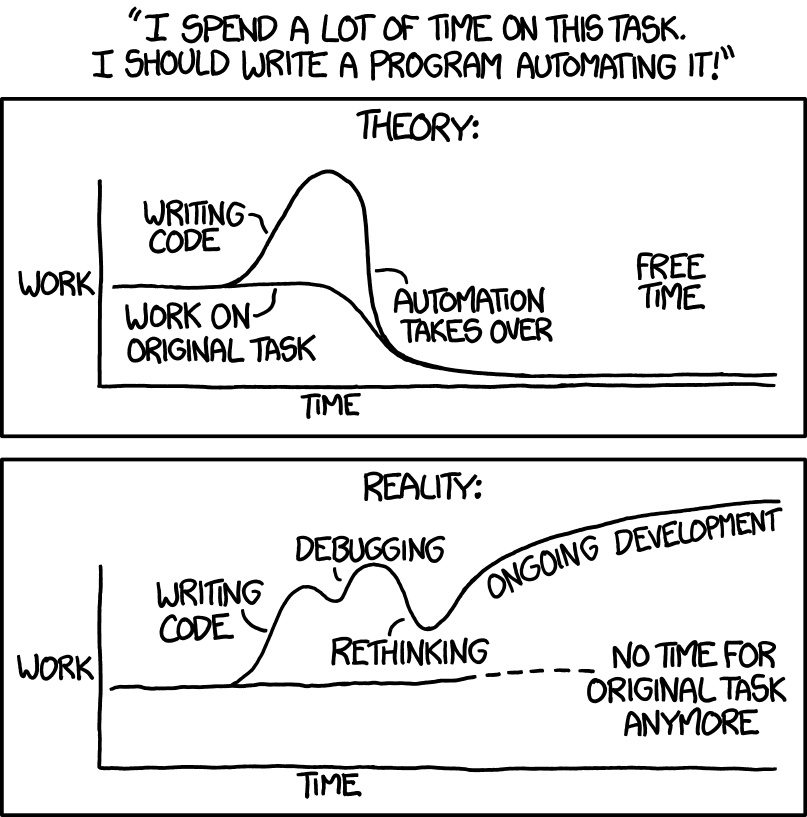
\includegraphics[width=0.4\linewidth]{automation_2x.png}
        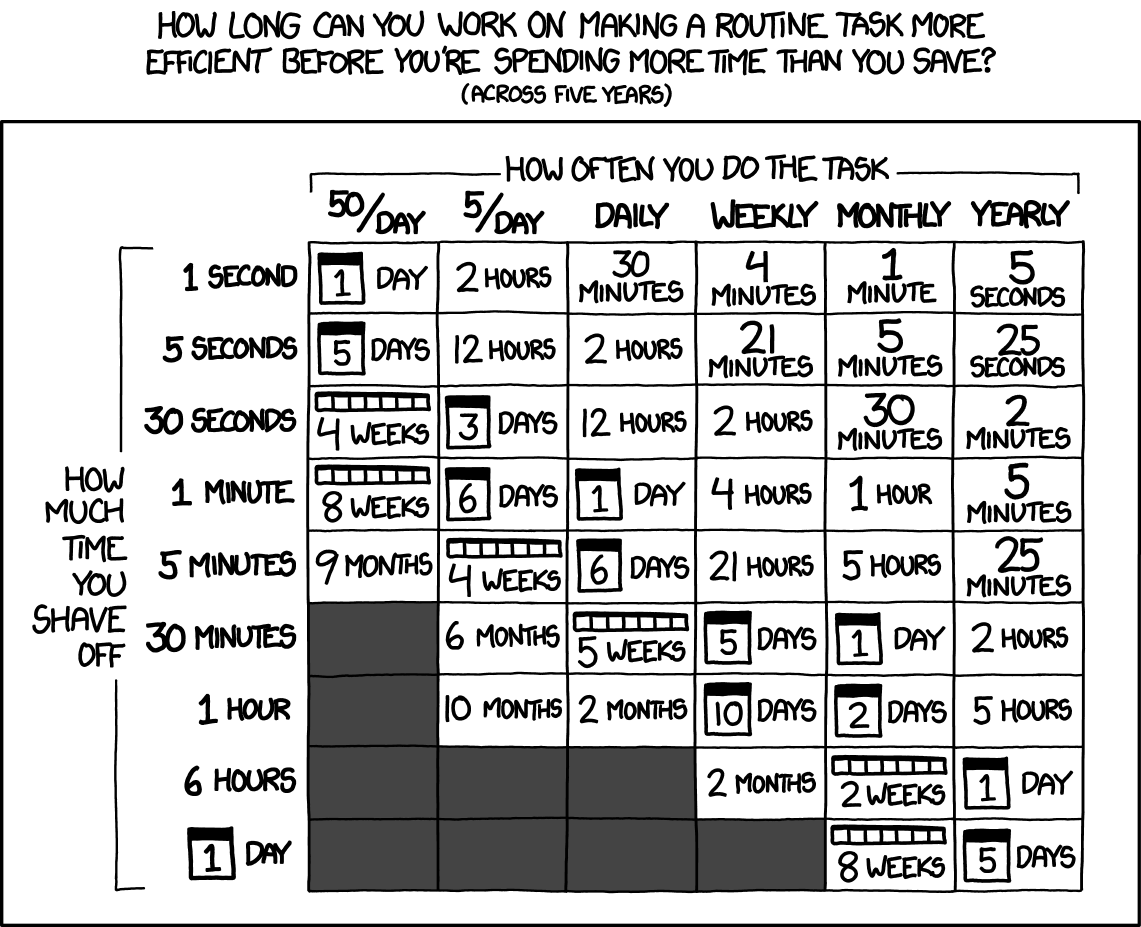
\includegraphics[width=0.5\linewidth]{is_it_worth_the_time_2x.png}
    \end{minipage}
\end{frame}

\begin{frame}[plain]
    \begin{minipage}{\textwidth}
        \centering
        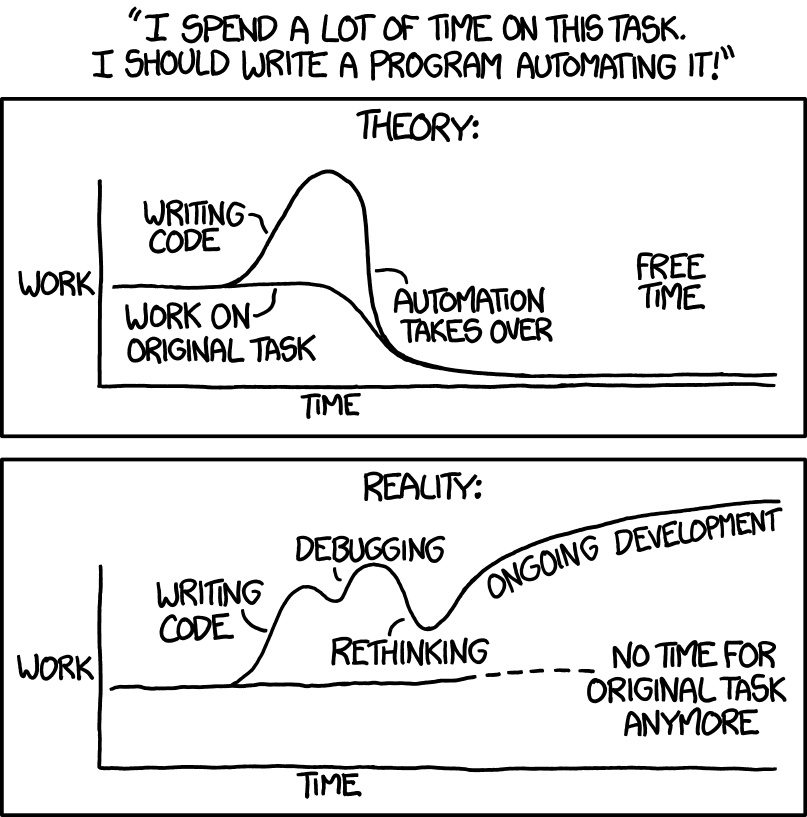
\includegraphics[width=0.4\linewidth]{automation_2x.png}
        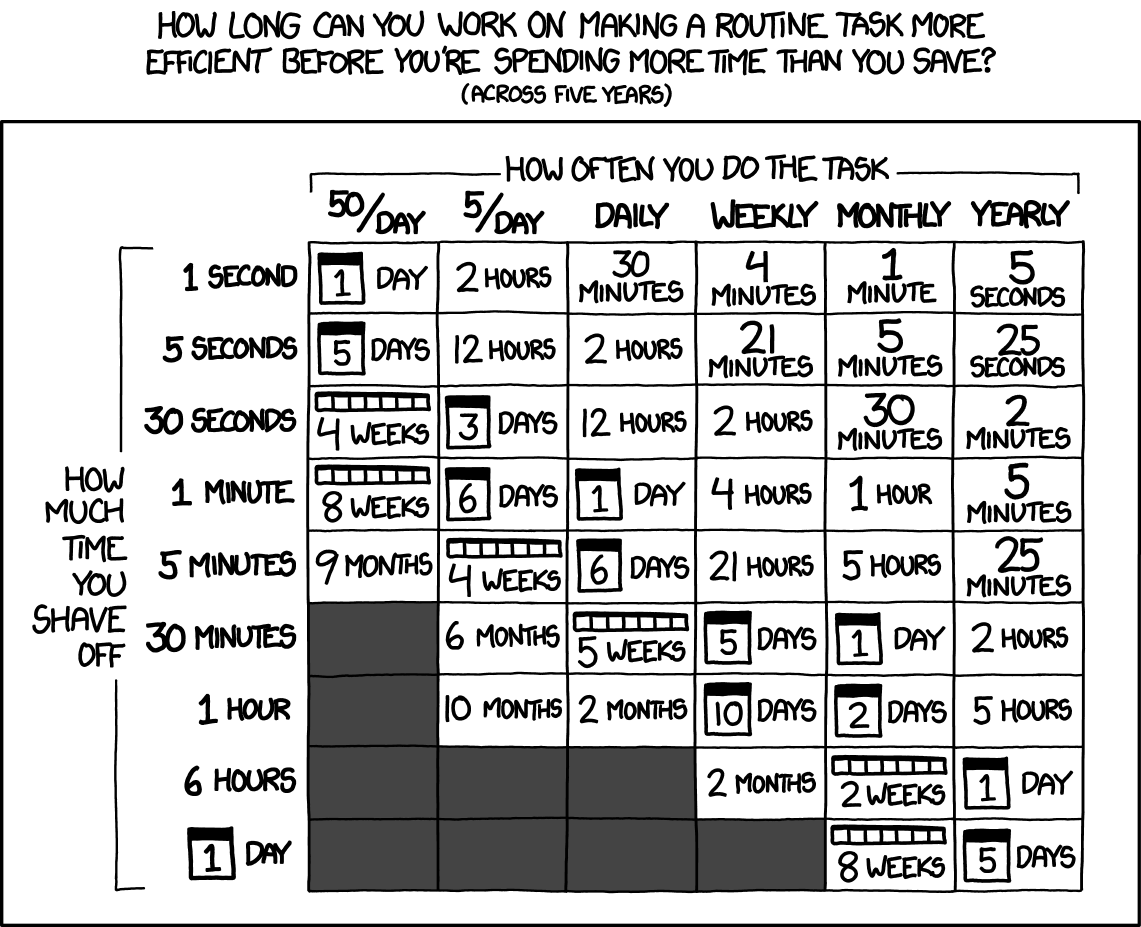
\includegraphics[width=0.5\linewidth]{is_it_worth_the_time_2x.png}
        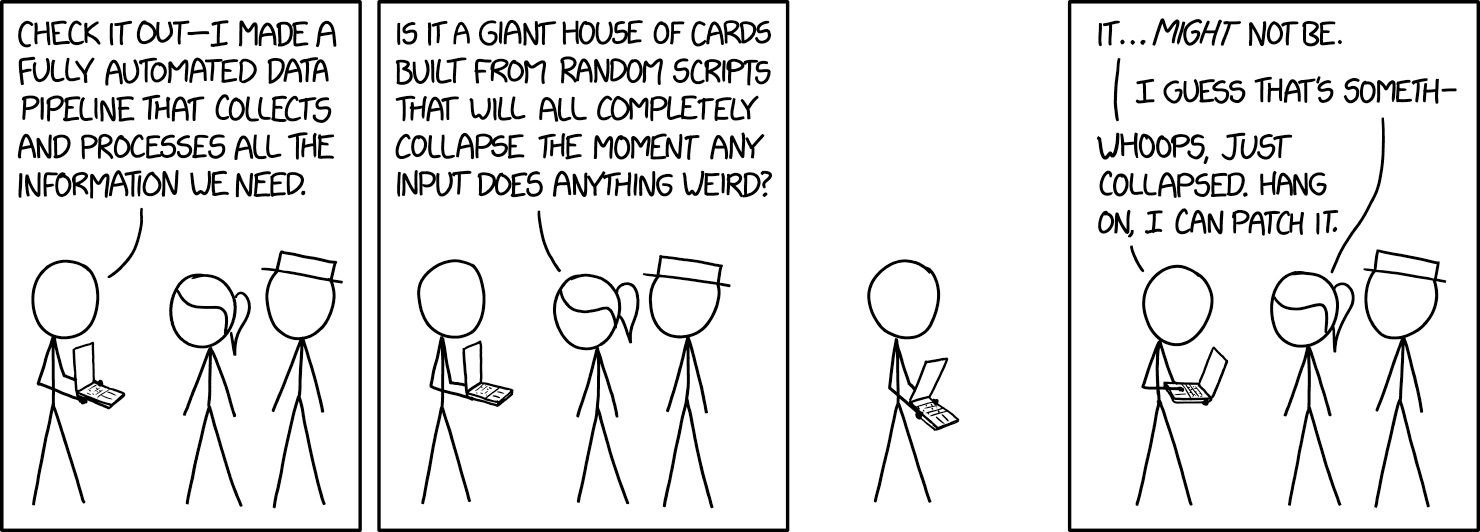
\includegraphics[width=0.47\linewidth]{data_pipeline_2x.png}
        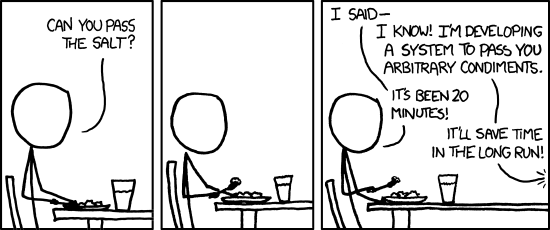
\includegraphics[width=0.4\linewidth]{the_general_problem.png}
        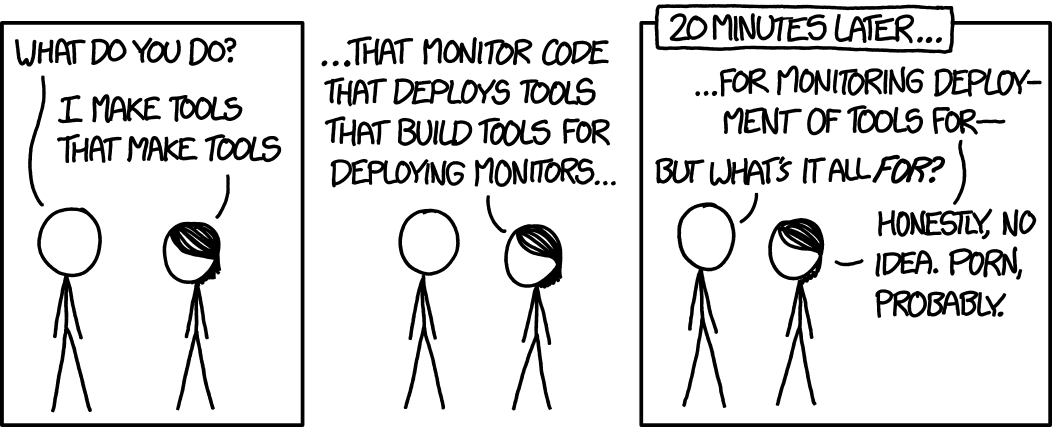
\includegraphics[width=0.4\linewidth]{tools_2x.png}
        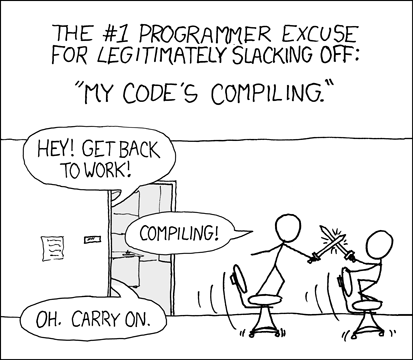
\includegraphics[width=0.2\linewidth]{compiling.png}
    \end{minipage}
\end{frame}


\section{How to Automate}

\begin{frame}{Github Actions}
    \begin{itemize}
        \item free product from Github for public repos
        \item ``on-demand'' VMs / containers
        \item triggered from git actions (push, pull request, etc)
        \item executions steps described in yaml
    \end{itemize}
\end{frame}

\begin{frame}[plain]
    \begin{minipage}{\textwidth}
        \centering
        \only<1>{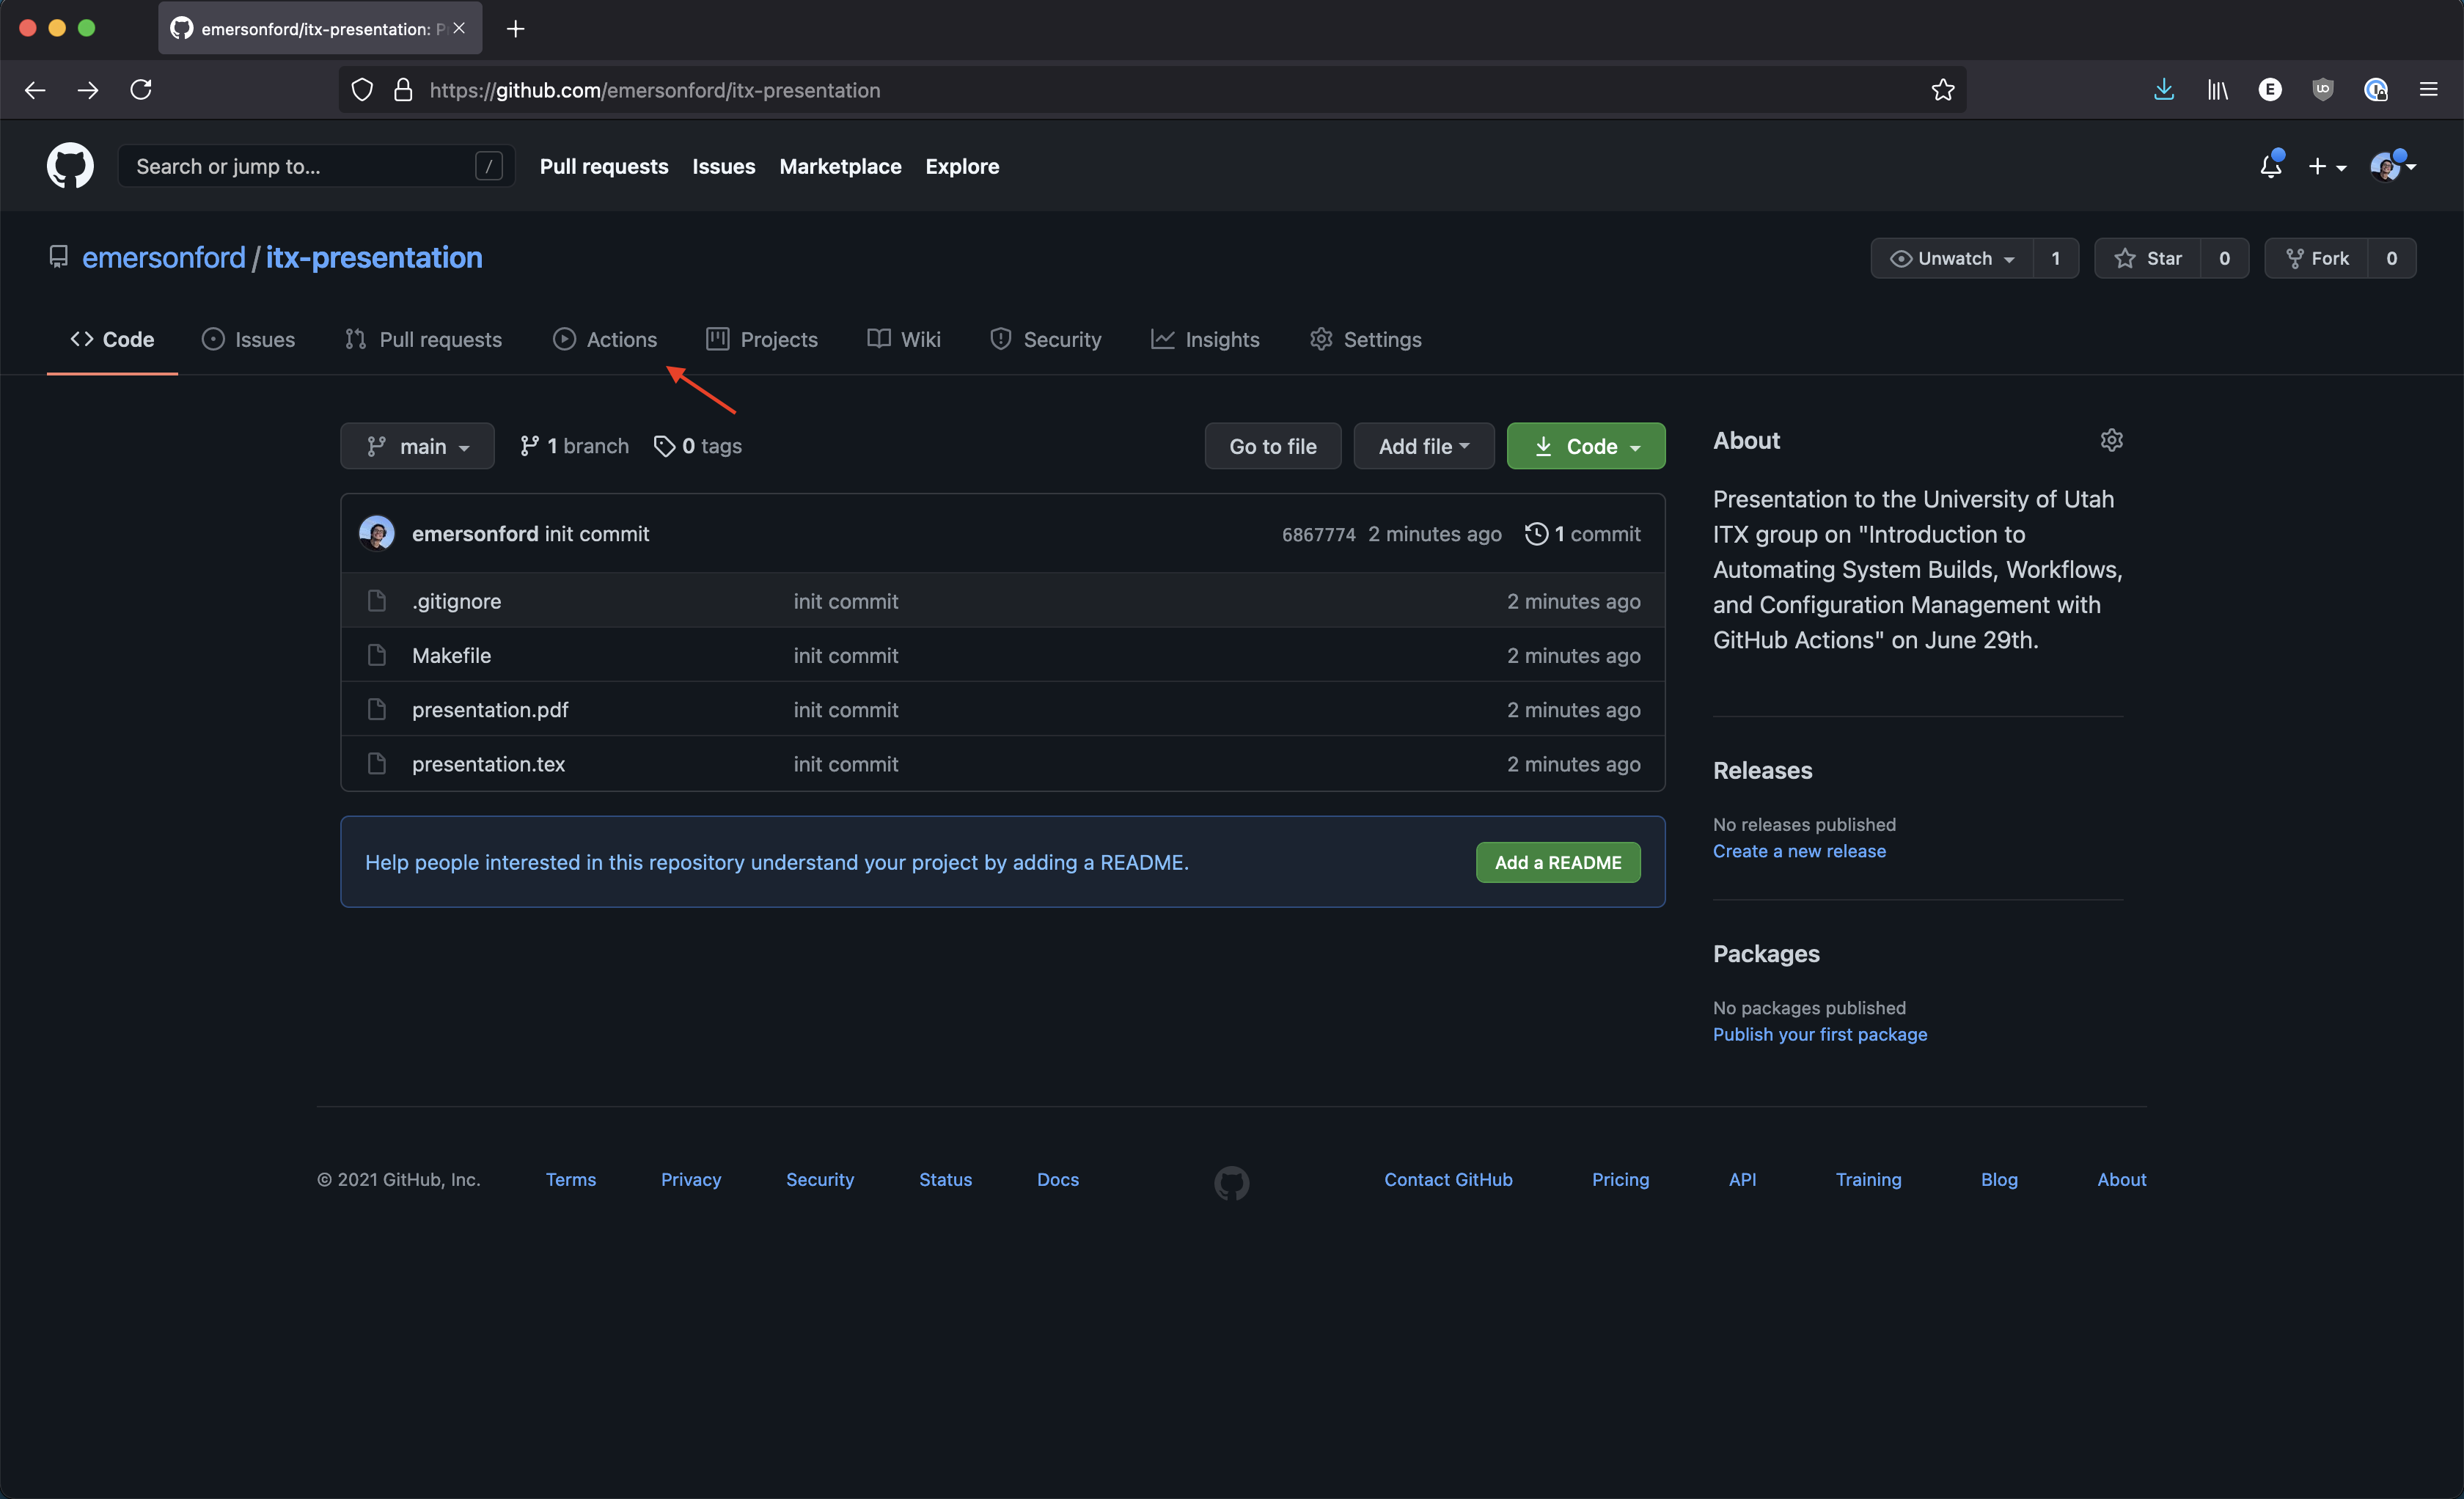
\includegraphics[width=\textwidth]{actions-getting-started1.png}}
        \only<2>{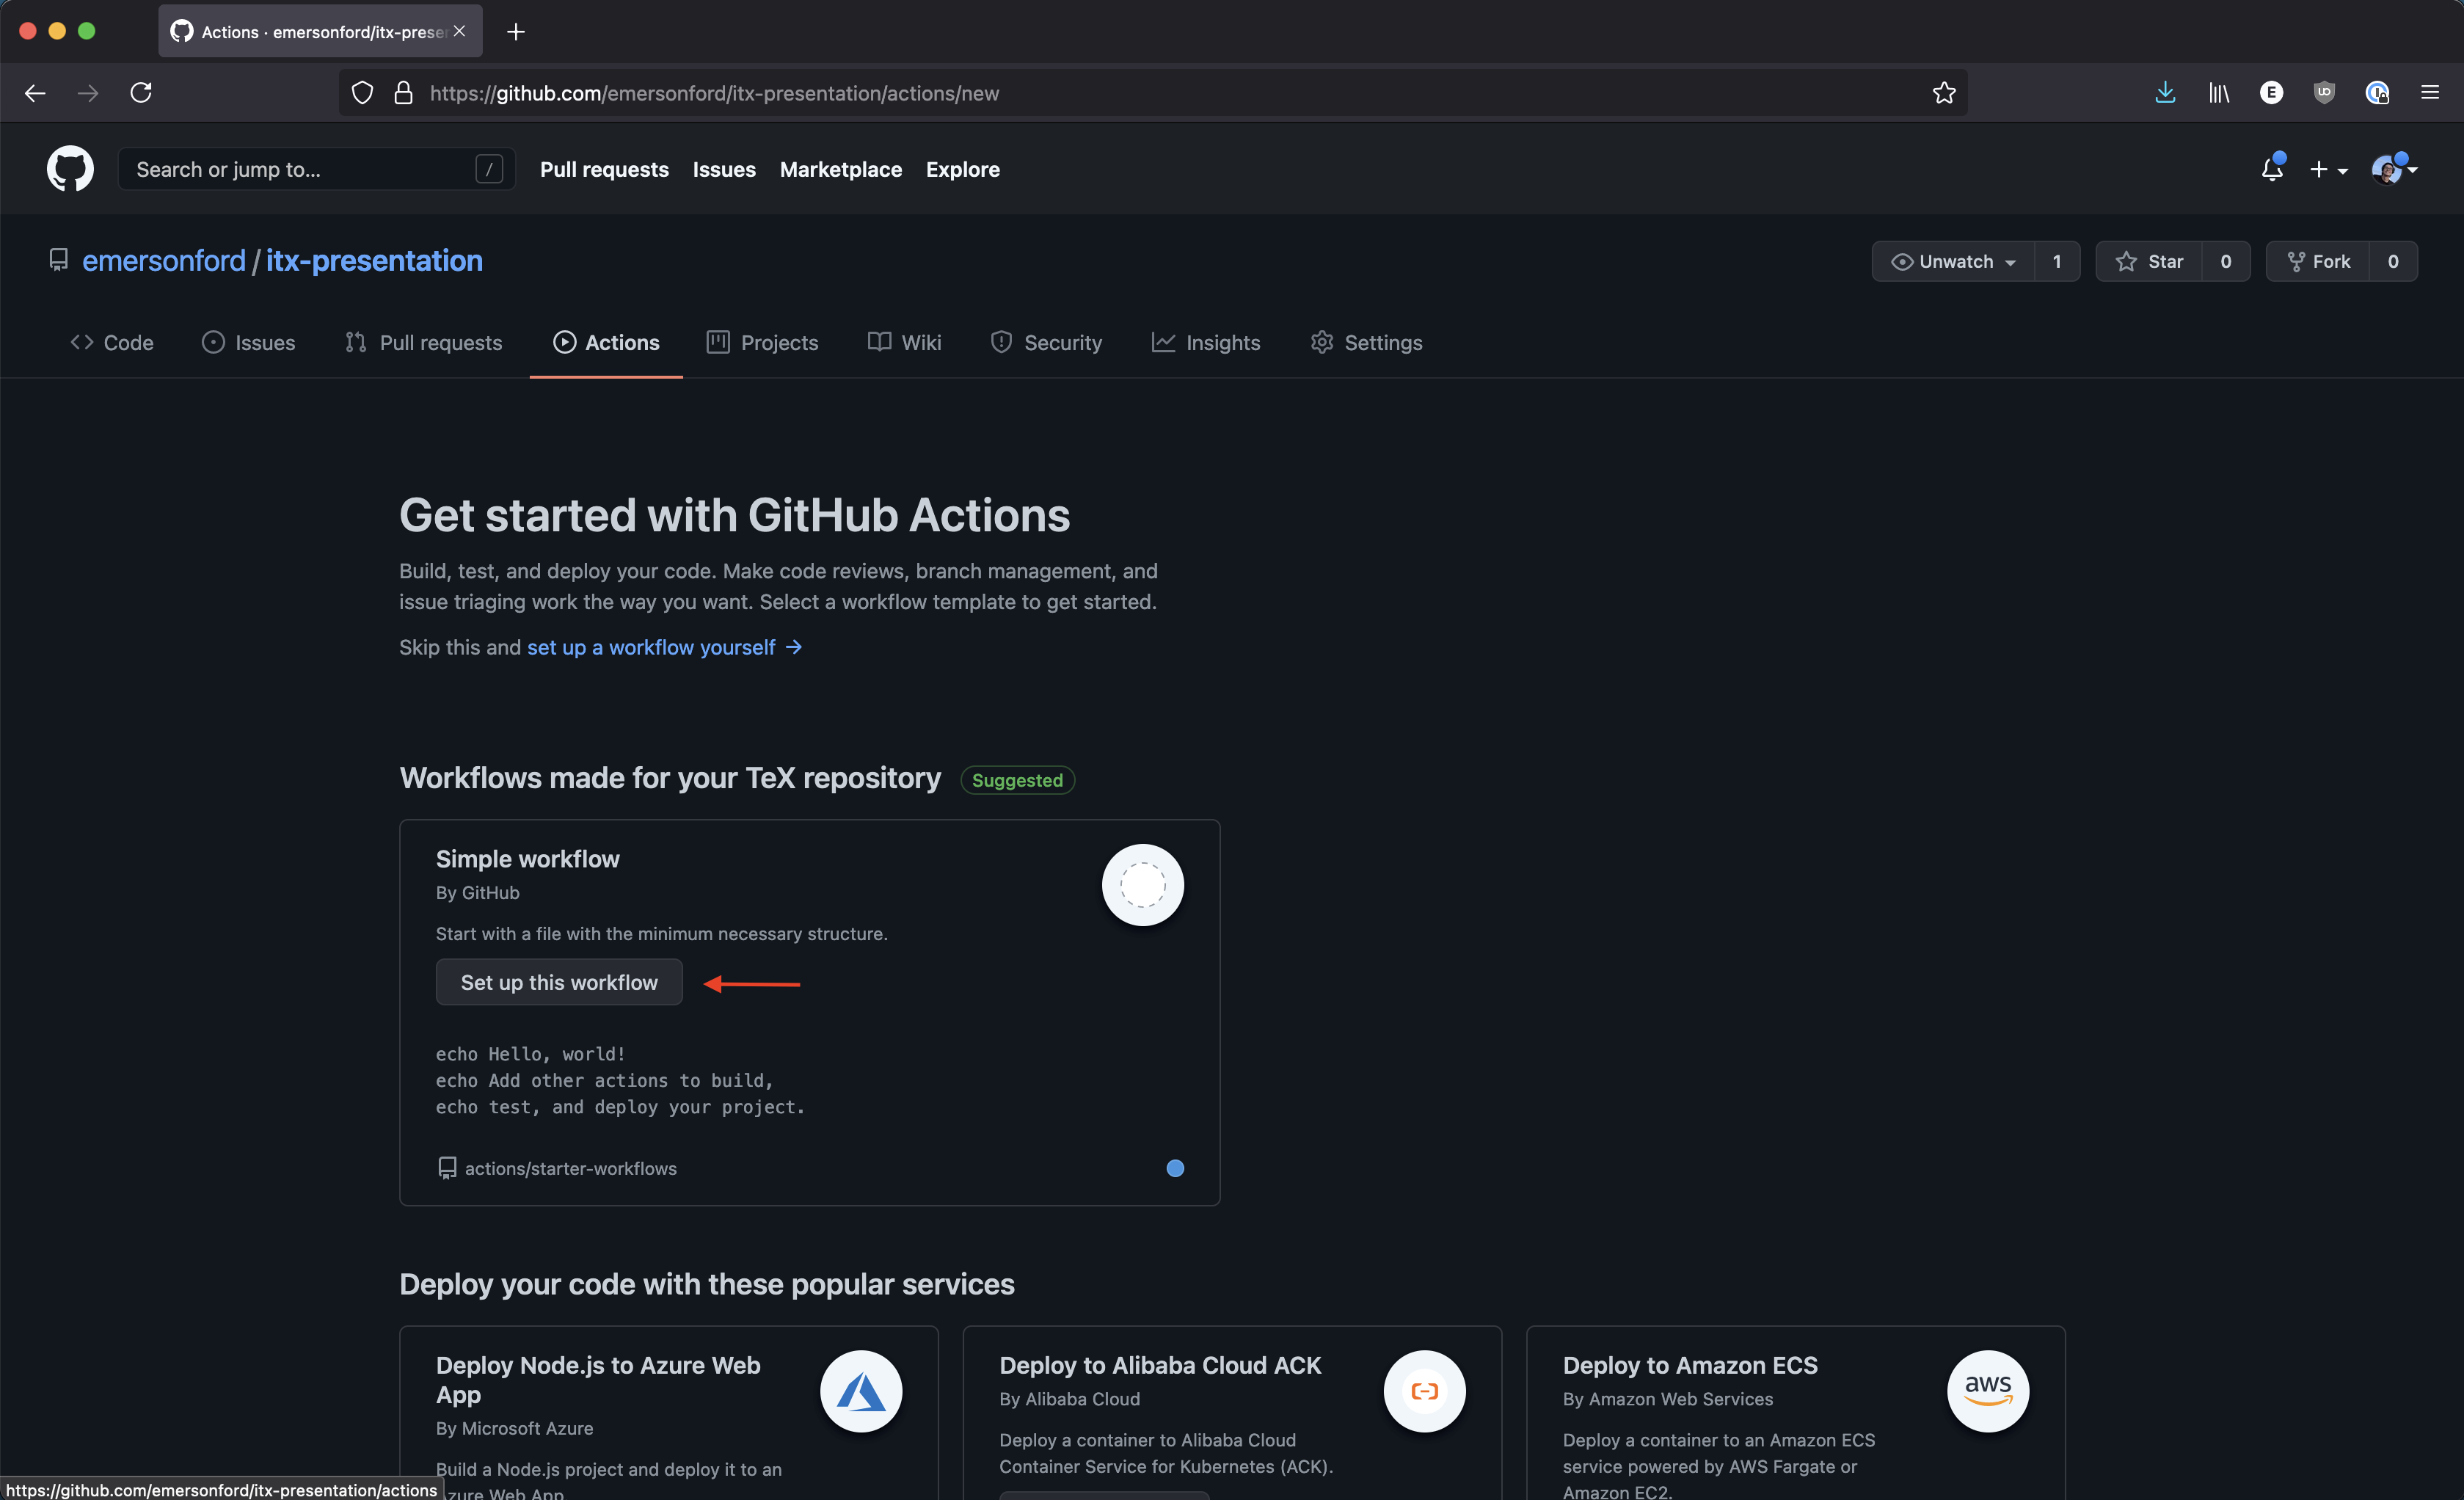
\includegraphics[width=\textwidth]{actions-getting-started2.png}}
        \only<3>{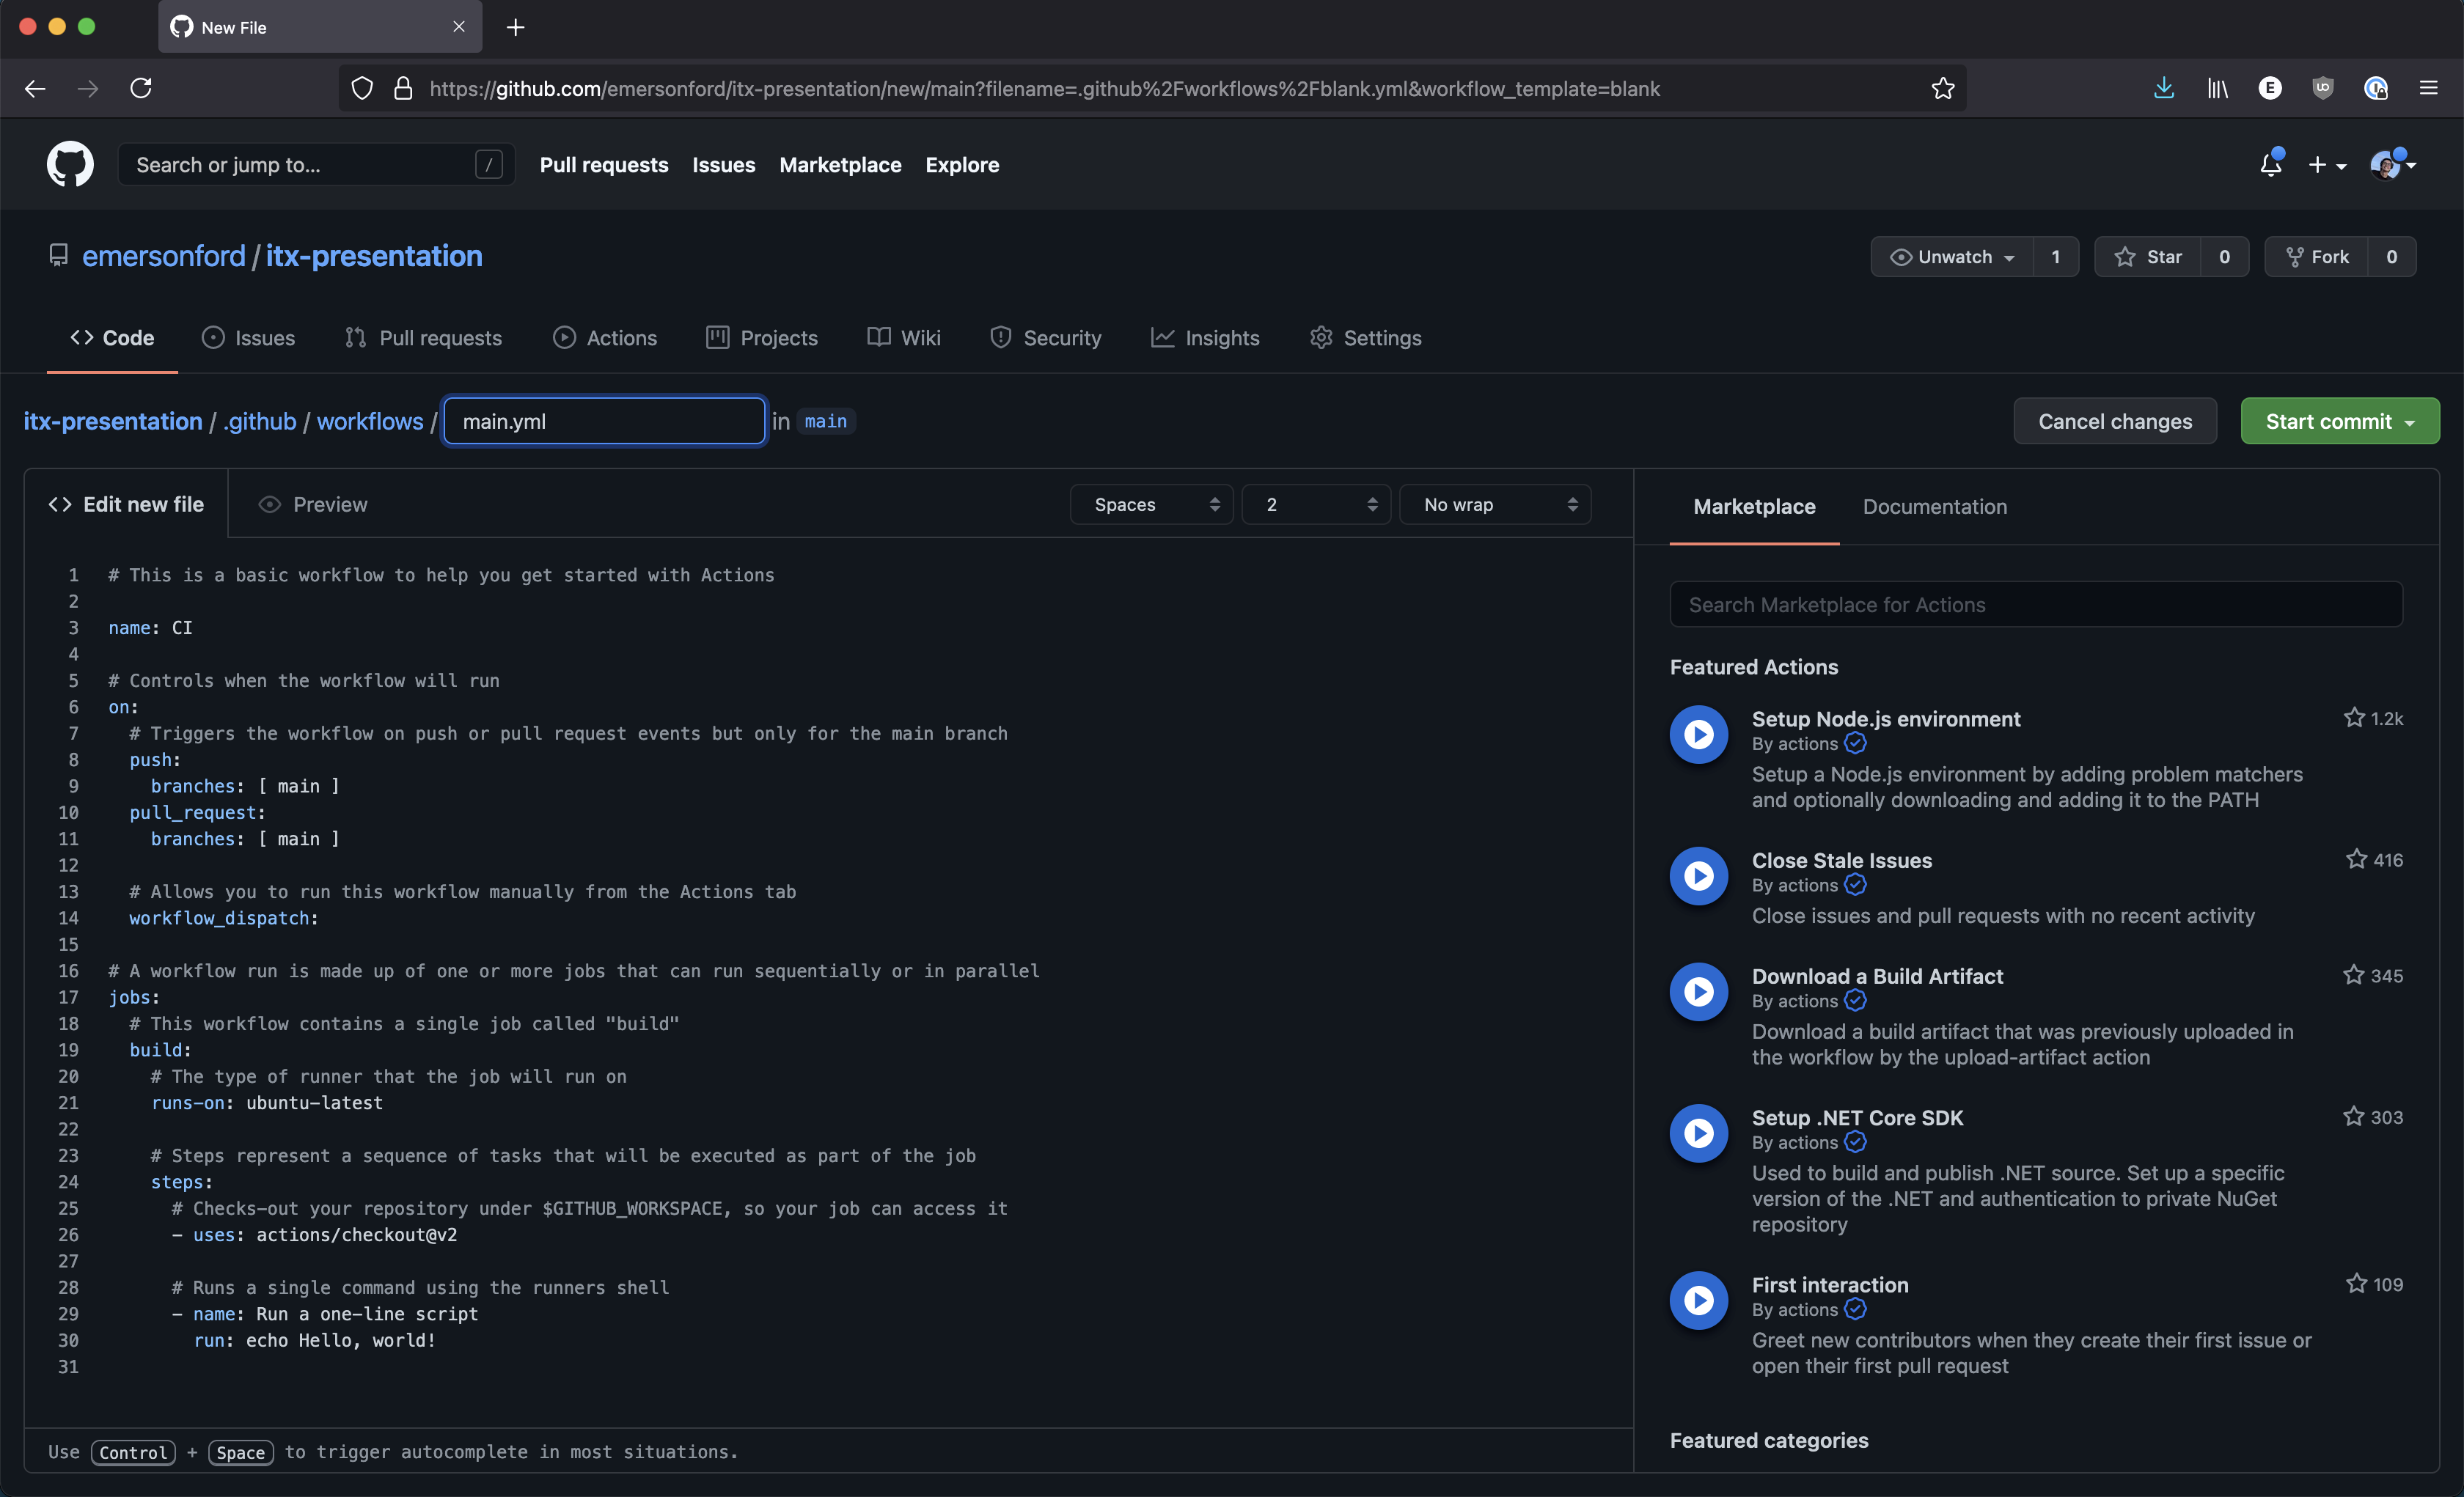
\includegraphics[width=\textwidth]{actions-getting-started3.png}}
    \end{minipage}
\end{frame}


\end{document}
